%!TEX root = ../main.tex
%
% フランク=ヘルツの実験
%


\section{フランク=ヘルツの実験}

\subsection{はじめに}

ボーアの量子論によると、原子の定常状態のエネルギーは離散的な値を持っていま 
す。エネルギーの一番低い状態を基底状態、エネルギーがその一つ上の定常状態を第 
一励起状態と呼びます。原子のエネルギーが離散的であることを、フランク=ヘルツの 
実験で確かめましょう。

1914年に、J.~フランクとG.~ヘルツは、ボーアの量子論を実験で証明し、この業
績によって1925年、ノーベル賞を受賞しました。

\subsection{測定原理}

ある原子の基底状態と、第一励起状態のエネルギーの差が$\Delta E$であったとします。
この原子のガスに加速させた電子を衝突させたとき、電子のエネルギーが$\Delta E$より小
さい場合は、原子は電子と弾性衝突を続け、それぞれの持つエネルギーは殆ど変化し
ません。しかし、電子のエネルギーが$\Delta E$より大きい場合は、原子は電子との衝突に
より$\Delta E$のエネルギーを受け取って第一励起状態に励起され、電子は$\Delta E$だけエネル
ギーを失うことになります。

%\begin{wrapfigure}[15]{r}{7cm}
%\vspace*{-0.8cm}
%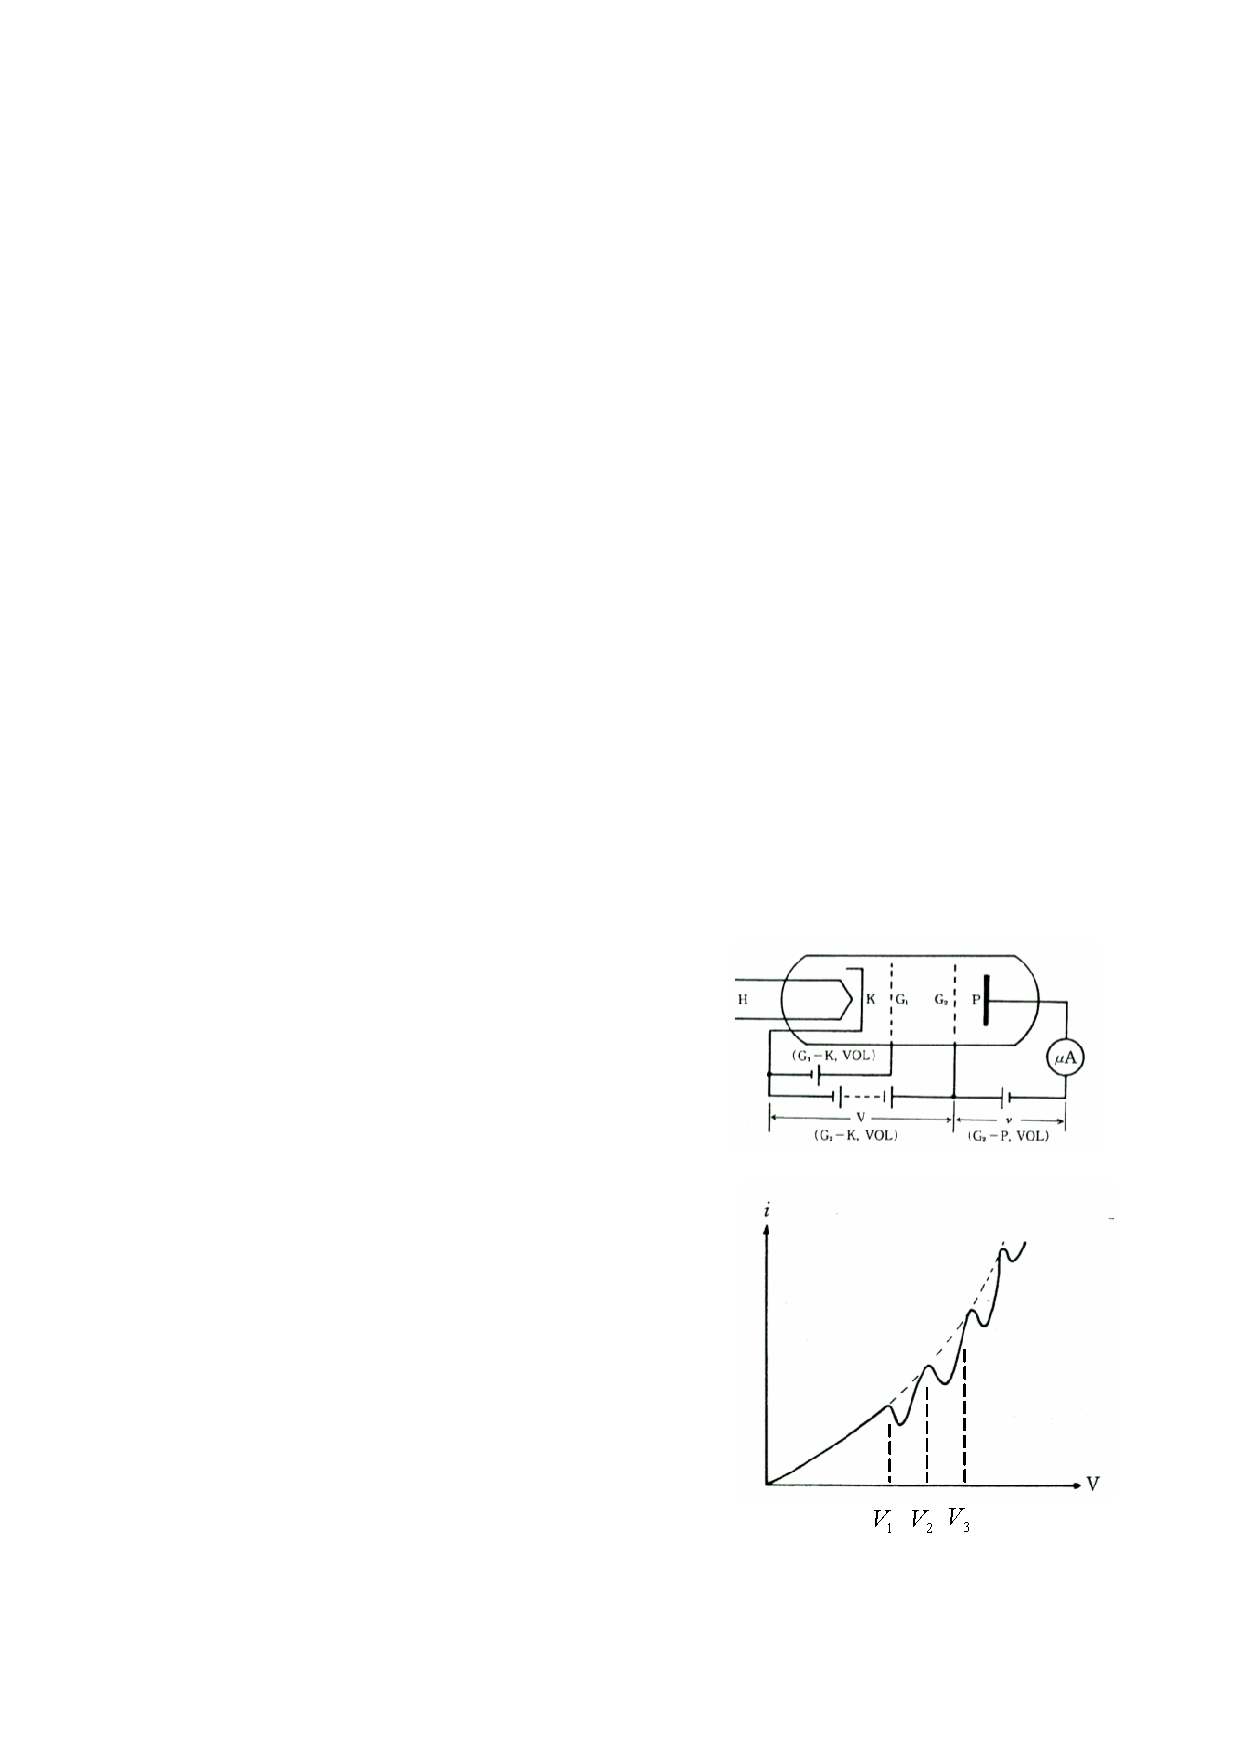
\includegraphics[scale=1.1]{FranckHertz/FranckHertz1.pdf}
%\end{wrapfigure}

実験では、図1のカソードKから放出した電 
子が、グリッド$\text{G}_1$までの間にかけられた電圧で 
加速され、グリッド$\text{G}_1$とグリッド$\text{G}_2$の間にあ 
る原子のガスに衝突します。グリッド$\text{G}_2$とプレ 
ートPの間には、電子を減速するための逆電圧を 
かけます。カソードKからグリッド$\text{G}_2$の間の電 
圧が小さい場合は電子と原子は弾性衝突をし、エ 
ネルギーを変化させずにグリッド$\text{G}_2$を通過してプ 
レートPに到着するため、プレートPに到着する電 
子はK-$\text{G}_2$間の電圧が上がるに従い増加します。 
しかし、K-$\text{G}_2$間の電圧を電子のエネルギーが$\Delta E$ 
を超えるまで大きくすると、原子を励起する衝突が 
起こるため、衝突した電子は$\text{G}_1$-$\text{G}_2$間で$\Delta E$だけ 
エネルギーを失って$\text{G}_2$を通過し、$\text{G}_2$-P間の逆電 
圧での減速によってプレートPに到達できなくなり、 
プレートPに到達する電子は一旦減少します。この減少を始める直前 
(ピーク時)のK-$\text{G}_2$間の電圧を$V_1$とします。

その後、電圧を上げていくと、プレートPに到達する電子はまた増加していきます
が、電圧が$V_1$の2倍を超えると$\text{G}_1$-$\text{G}_2$間で二回原子を励起する衝突ができるように
なるため、$\Delta E$の2倍のエネルギーを失うことになり、プレートPに到達する電子は
再び減少します。その後も同様に、 $V_1$の整数倍の電圧の所で、Pに到達する電子の量
が一旦減少を始めることになります。(図2)

\begin{figure}[t]
\begin{tabular}{cc}
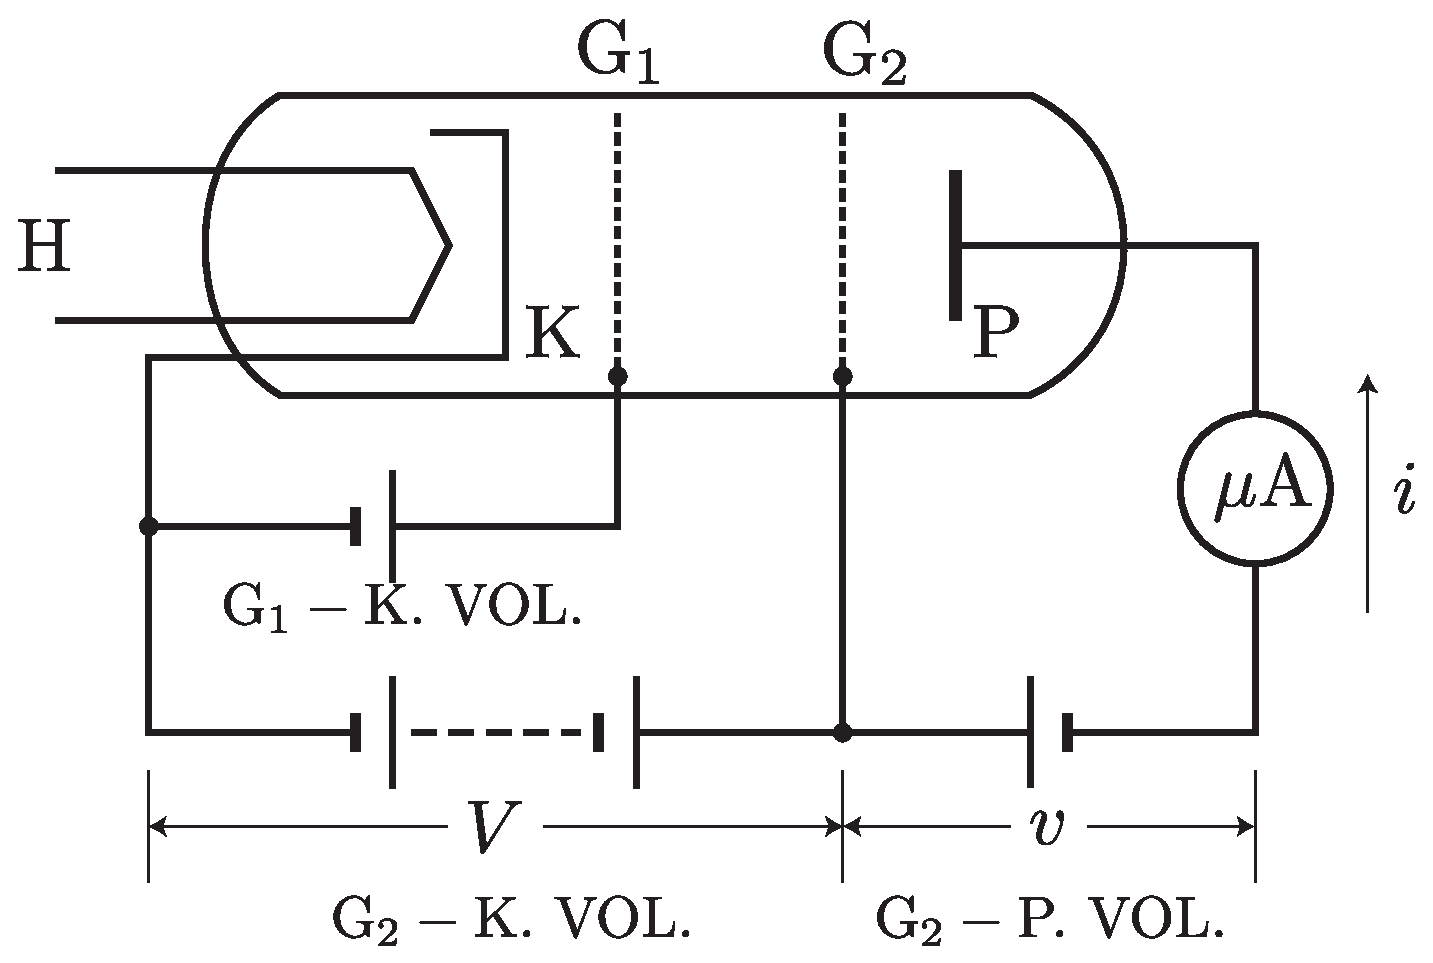
\includegraphics[scale=0.35]{13_FranckHertz/franckhertz.eps} & 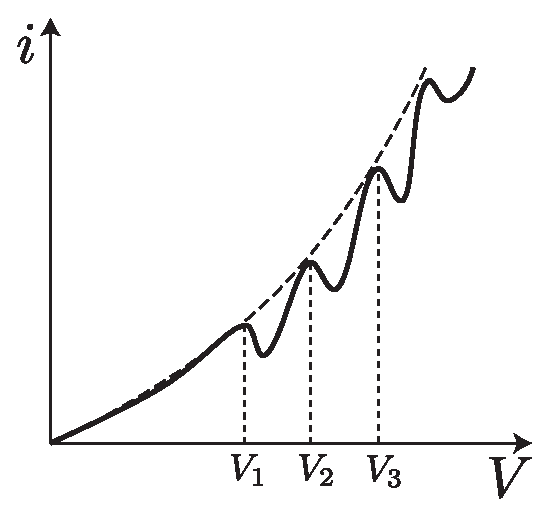
\includegraphics[scale=0.63]{13_FranckHertz/plot.eps}\\
図1: フランク=ヘルツ実験器の回路図 & 図2:グリッド電圧とプレート電流
\end{tabular}
\end{figure}


この原理より、原子の励起エネルギー$\Delta E$は次の式で求められます。
\[
\Delta E = V_{n+1}-V_n \quad \text{[eV]}
\]
$V_n$を測定し、上の式から原子の励起エネルギーを計算しましょう。


\newpage

\jikken

\begin{itemsquarebox}[c]{\bf 実験用具}
フランク=ヘルツ実験器、電圧計、電流計、グラフ用紙
\end{itemsquarebox}

\bigskip

\subjikken{原子の励起電圧の測定}

\begin{enumerate}

\item ここで使用するフランク=ヘルツ実験器の真空管は、ネオンガスが入った真空管
です。実験装置の説明書に従って、電圧計と電流計を実験装置に接続します。
フランク=ヘルツ実験器にも電圧計と電流計は内蔵されていますが、
電圧と電流をより正確に読み取るために、外部に接続した電圧計と電流計を用います。

\item 実験装置の説明書に書かれた手順をよく読み、装置の調整を行った後、加
速電圧を2 [V]ずつ増やしながら、加速電圧$V$とプレート電流$i$の値を読み取って
いきます。結果は、横軸を加速電圧、縦軸をプレート電流に取り、グラフにプロ
ットし、なめらかな曲線でつなぎましょう。

\item グラフの山(ピーク時)の部分の電圧を読み取り、ネオン原子の励起電圧を求めましょう。



\end{enumerate}

\paragraph{注意}
加速電圧は少しずつ上げていき、プレート電流の針が右に振り切れることの 
ないように気をつけましょう。また、\underline{プレート電流の針が振り切れた場合は、 
ただちに}\\\underline{加速電圧をゼロに戻してください。}


